\documentclass[10pt]{article}
%\usepackage[utf8]{inputenc} % Under score not copyable
\usepackage[T1]{fontenc}
\usepackage{geometry}
 \geometry{
 a4paper,
 total={170mm,257mm},
 left=20mm,
 top=20mm,
 }
 \usepackage{graphicx}
 
\setlength\parindent{0pt}

\title{Clang Code Standard Plugins}
\author{Job Mensen \& Richard Faasse}
\date{\today}

\usepackage{natbib}
\usepackage{graphicx}
\usepackage{hyperref}
\usepackage{xcolor}

\begin{document}

\maketitle
\noindent This document shows the steps needed to install the tooling used in this project to enforce code standards.

\section{Clean code (beautifier}
It is decided to use style tooling for formatting the C++ code. This is chosen so that developers don't need to worry about style issues.

\subsection*{Install Clang-Format}
In Linux, open your \textbf{terminal}, and type in \texttt{sudo apt install clang-format}

\subsection*{Implementation for your IDE}
\subsubsection*{A) Plugin in Qt Creator}
\begin{enumerate}
\item Open Qt Creator (version 4.12.0 or later), go to \textbf{Help}, and select \textbf{About Plugins...}
\begin{figure}[h!]
\centering
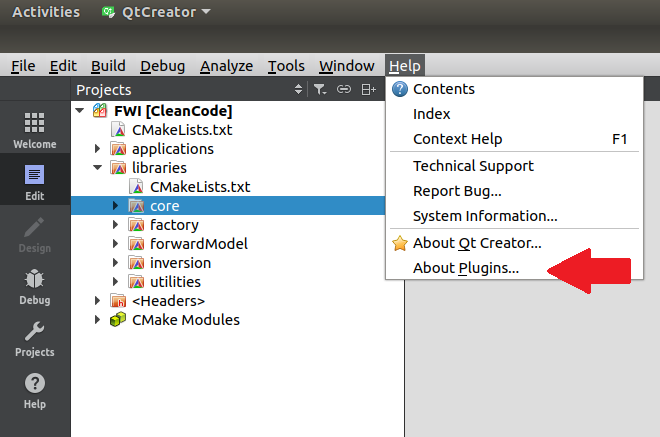
\includegraphics[width=0.6 \textwidth]{clang-format1.png}
\end{figure}

\newpage

\item Select \textbf{Beautifier (experimental)} under C++, and \textbf{close} Qt Creator.
\begin{figure}[h]
\centering
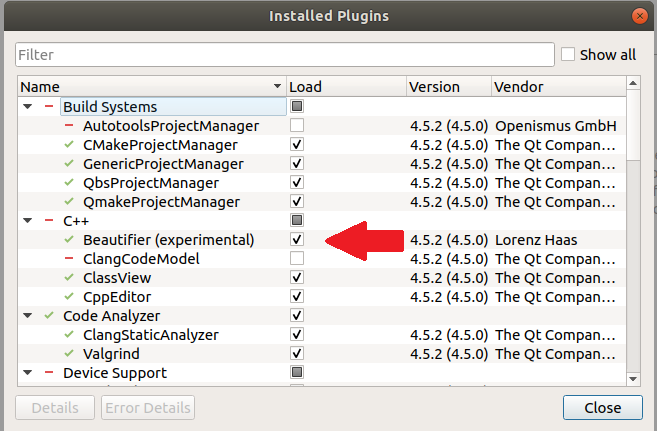
\includegraphics[width=0.6 \textwidth]{clang-format2.png}
\end{figure}

\item Open Qt Creator, go to \textbf{Tools}, and select \textbf{Options...}
\begin{figure}[h!]
\centering
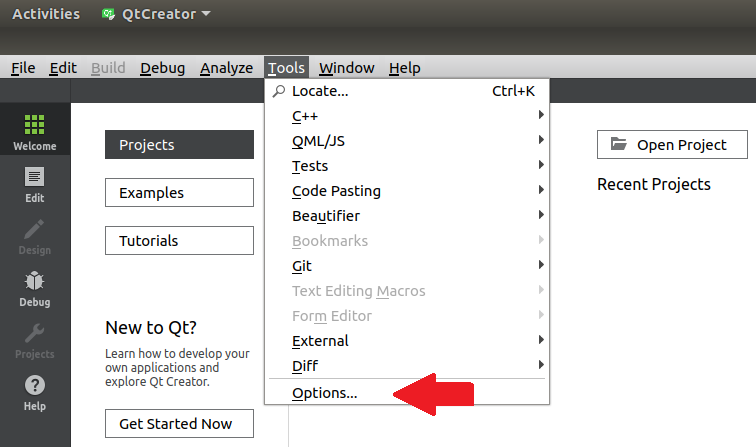
\includegraphics[width=0.6 \textwidth]{clang-format3.png}
\end{figure}

\item In \textbf{Options} select \textbf{Beautifier} (1). In the \textbf{General} tab, check \textbf{Enable auto format on File Save} (2),
select \textbf{ClangFomat} (3), and check \textbf{Restrict to files contained in the current poject} (4).
\begin{figure}[h!]
\centering
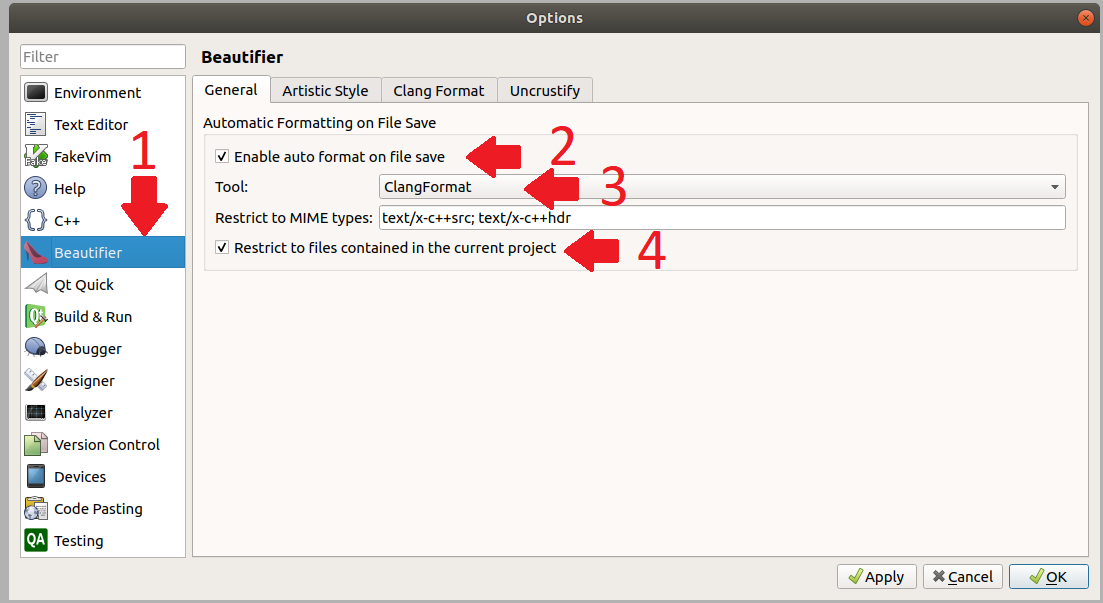
\includegraphics[width=0.7 \textwidth]{clang-format4.png}
\end{figure}

\newpage

\item In this window select tab \textbf{Clang Format} (1). Verify if \textbf{Clang Format command} (2) is correctly
filled in. Select option \textbf{File} in \textbf{Use predefined style} (3) and select \textbf{None} as \textbf{Fallback style} (4).
Note: Clang-Format automatically searches for the .clang-format file in the (parent) directory.
\begin{figure}[h!]
\centering
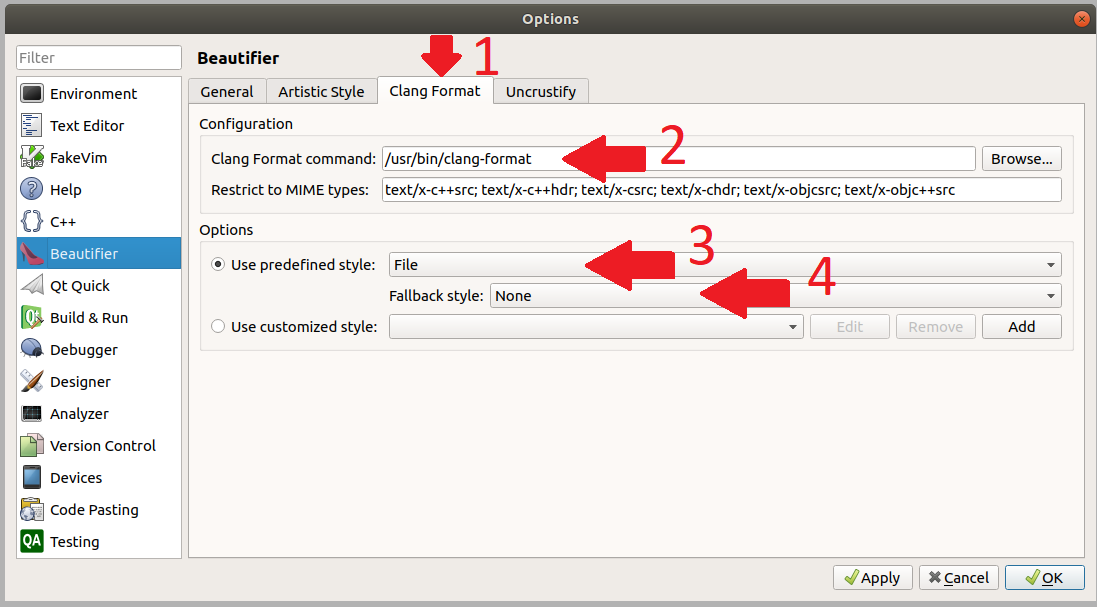
\includegraphics[width=0.7 \textwidth]{clang-format5.png}
\end{figure}
\end{enumerate}

\subsubsection*{B) CLang Format in other IDE's}
In most IDE’s a Clang-format plugin is available that works in a similar way as described above. It is important to select predefined style by file. Clang-Format will then automatically search the style format file. 

\subsection*{Change the style format}
The style used by Clang-Format is implemented in the .clang-format file in the parallelized-fwi folder. This file has no name, and is thus simply called .clang-format. In Ubuntu it is a hidden file, but it can be shown by clicking \textbf{Crtl + H}. Note: the version of Clang-Format is decisive for commands that can be used. Unfortunately, some commands had to be removed.
\newpage

\section{Code-standards (Naming \& Good practice)}
For the enforcing of code standards, clang-tidy is used, which gives IDE warnings when code-standard criteria are not met. These standards themselves are described in the CodeStandards documentation in this project (found in the README folder).

\subsection*{Install clang-tidy}
Run the following command in your Linux terminal: \texttt{sudo apt install clang-tidy}

\subsection*{Implementation for your IDE}
\subsubsection*{A) Plugin in Qt Creator}

\begin{enumerate}
\item To enable the clang-tidy plugin into the Qt Creator IDE, first go to \textbf{Help} $\rightarrow$ \textbf{About Plugins...}
\begin{figure}[h!]
\centering
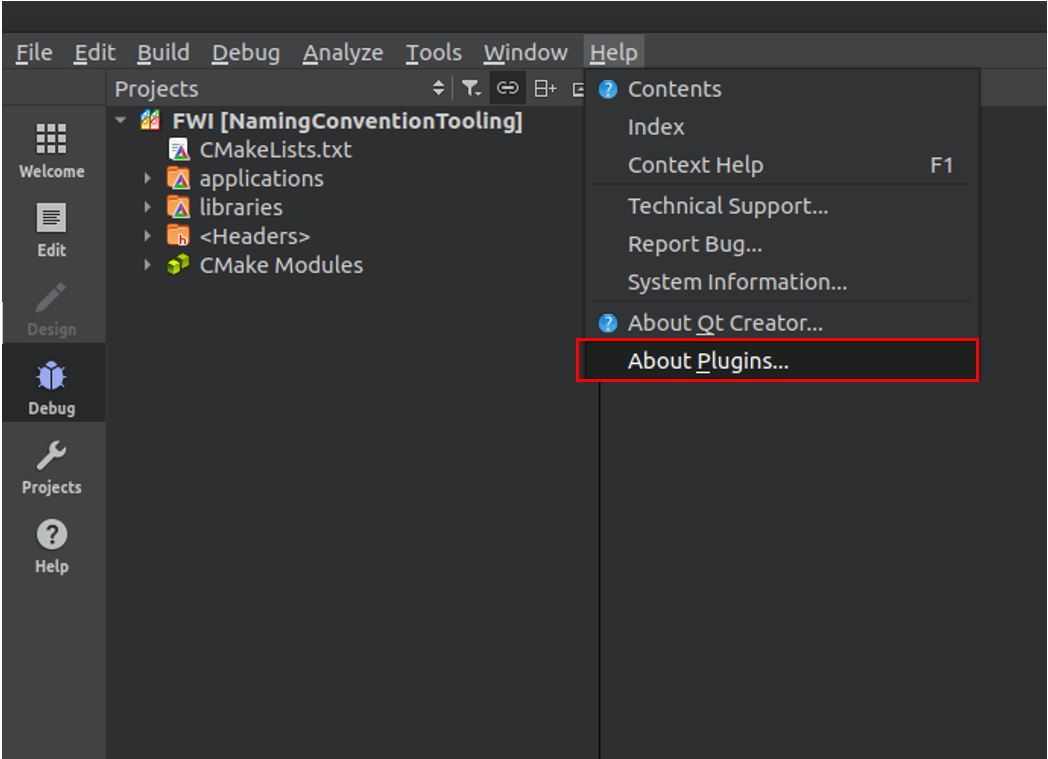
\includegraphics[width=0.6 \textwidth]{clang-tidy1.png}
\end{figure}

\item Tick the box next to the \textbf{ClangCodeModel} if this was not already the case.
\begin{figure}[h!]
\centering
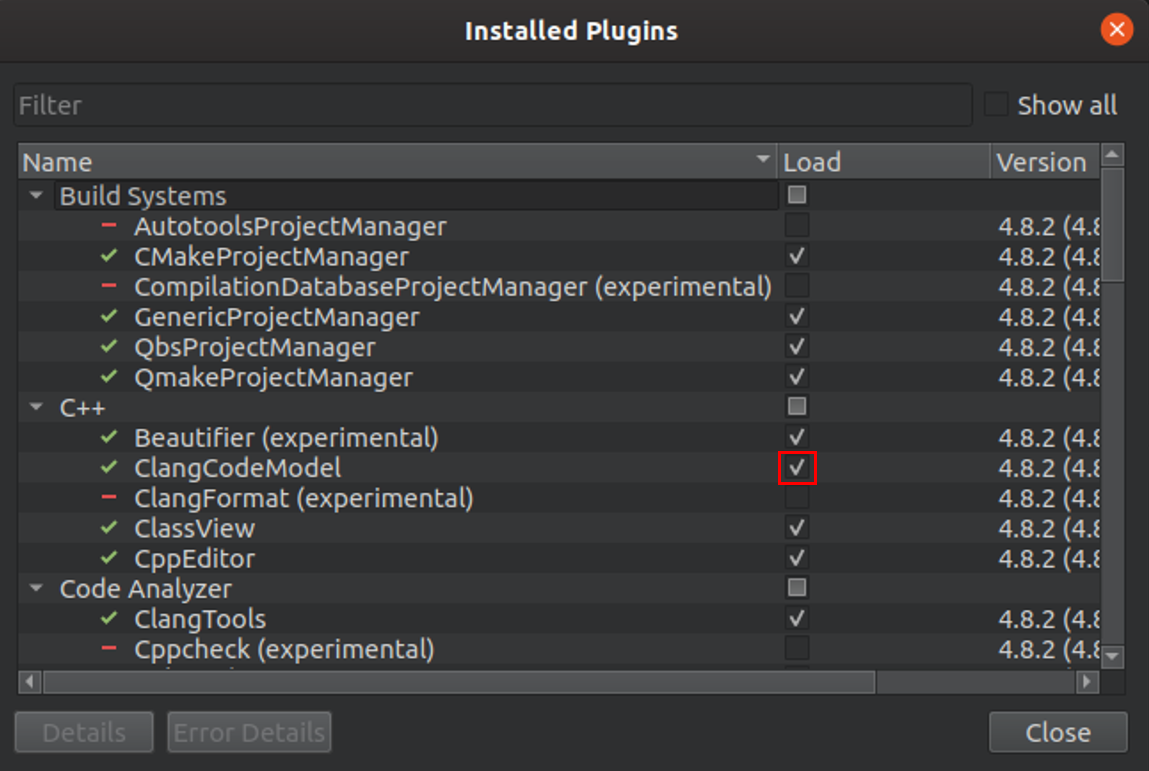
\includegraphics[width=0.6 \textwidth]{clang-tidy2.png}
\end{figure}

\newpage

\item Having done this, go to \textbf{Tools} $\rightarrow$ \textbf{Options}
\begin{figure}[h!]
\centering
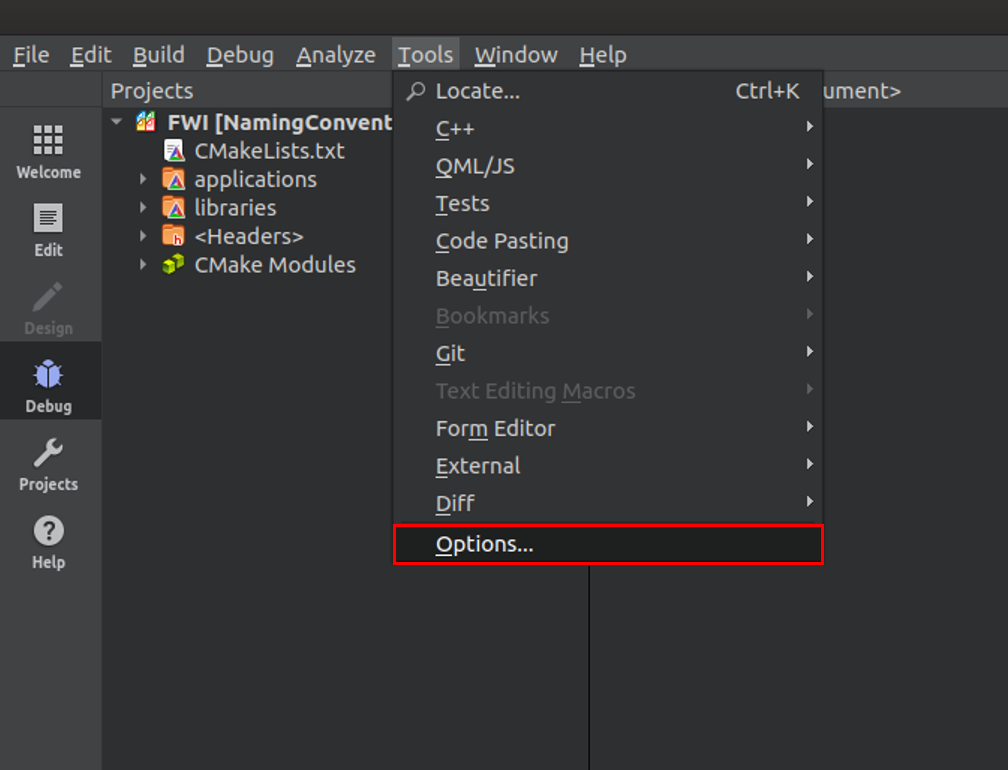
\includegraphics[width=0.6 \textwidth]{clang-tidy3.png}
\end{figure}


\item In the options, go to \textbf{Analyzer} and to the \textbf{Clang Tools} tab.
\begin{figure}[h!]
\centering
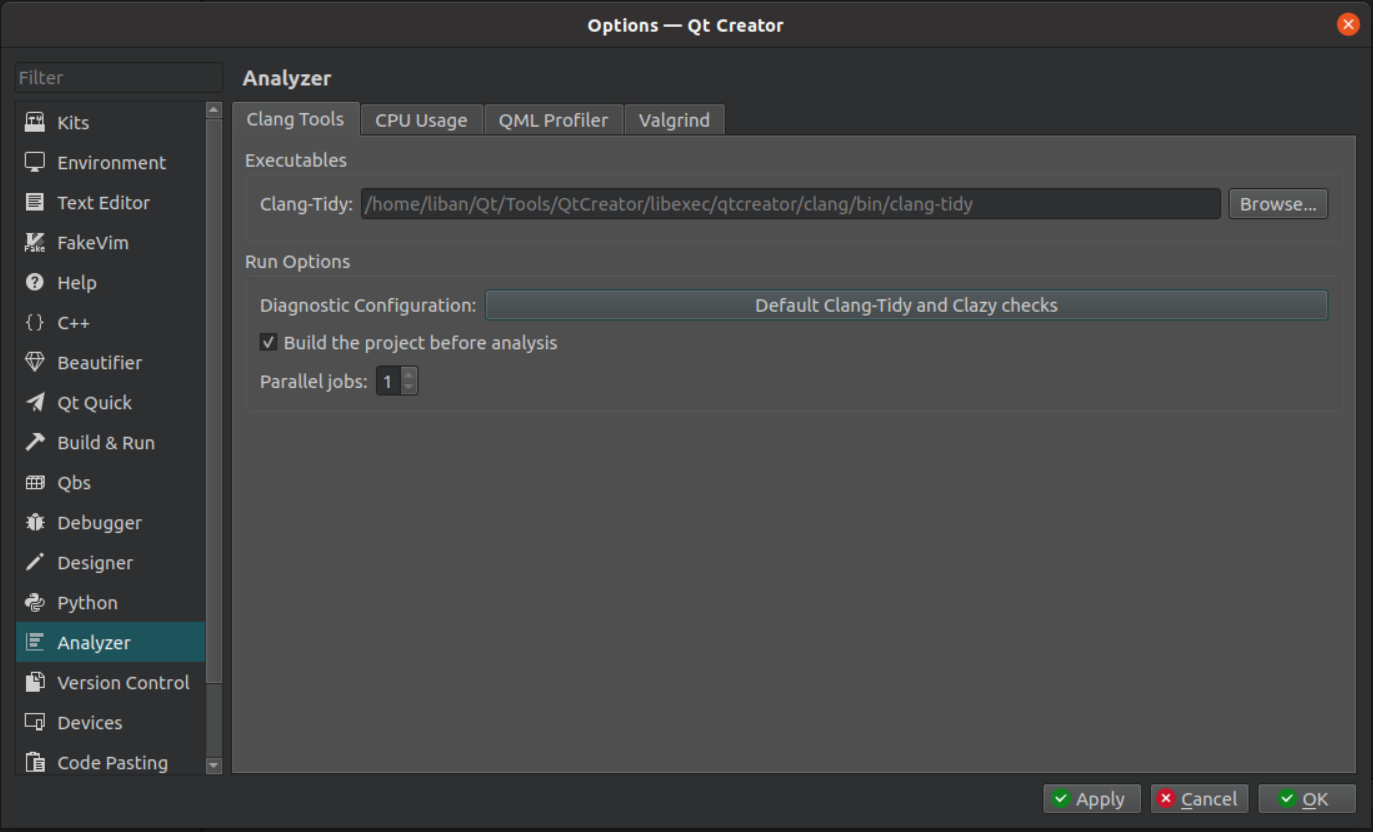
\includegraphics[width=0.6 \textwidth]{clang-tidy4.png}
\end{figure}

\item Next select Diagnostic Configuration by clicking on \textbf{Default Clang-Tidy and Clazy Checks} option.
\begin{figure}[h!]
\centering
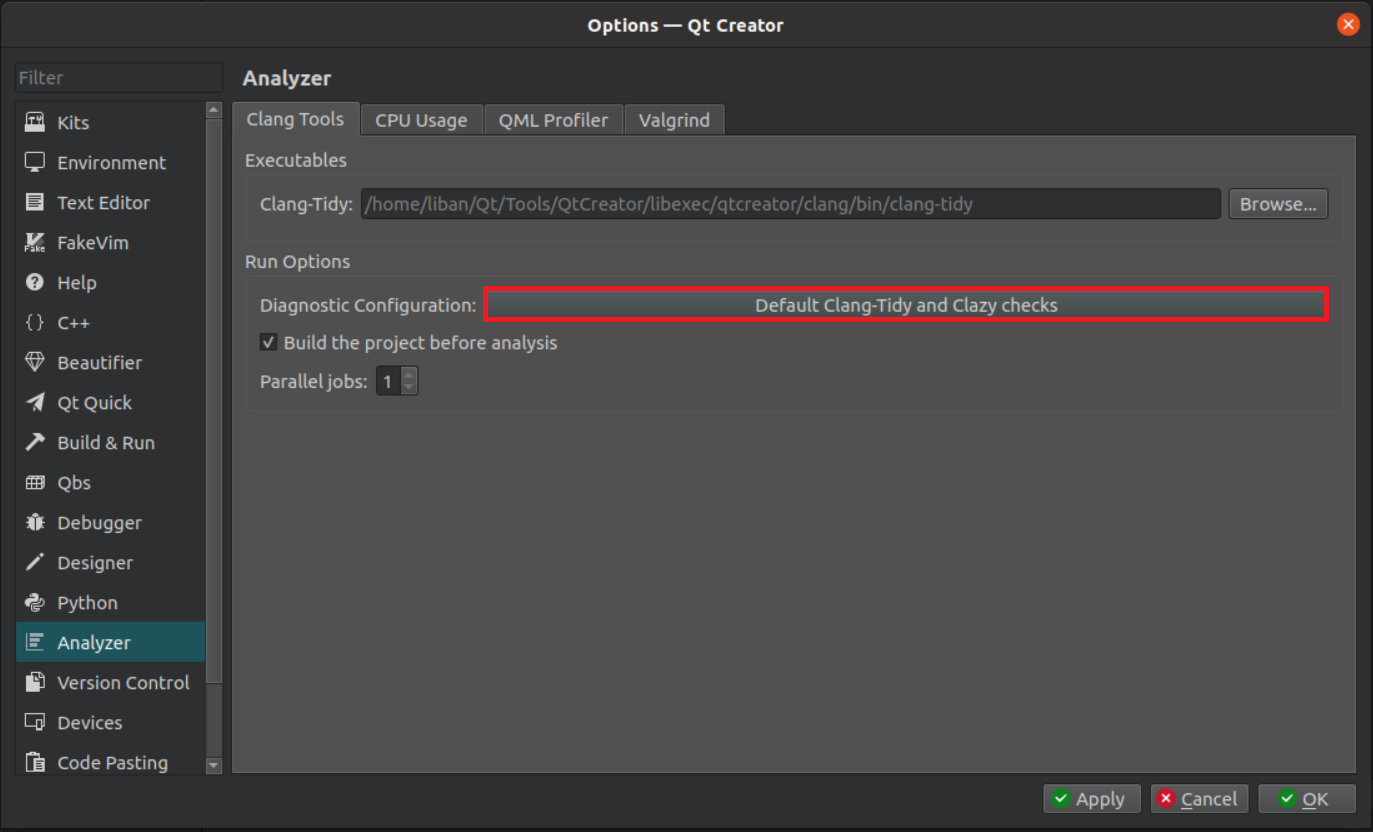
\includegraphics[width=0.7 \textwidth]{clang-tidy5.png}
\end{figure}

\item Select \textbf{Default Clang-Tidy and Clazy checks} and press \textbf{Copy} to be able to customize it
and give it a suitable name.
\begin{figure}[h!]
\centering
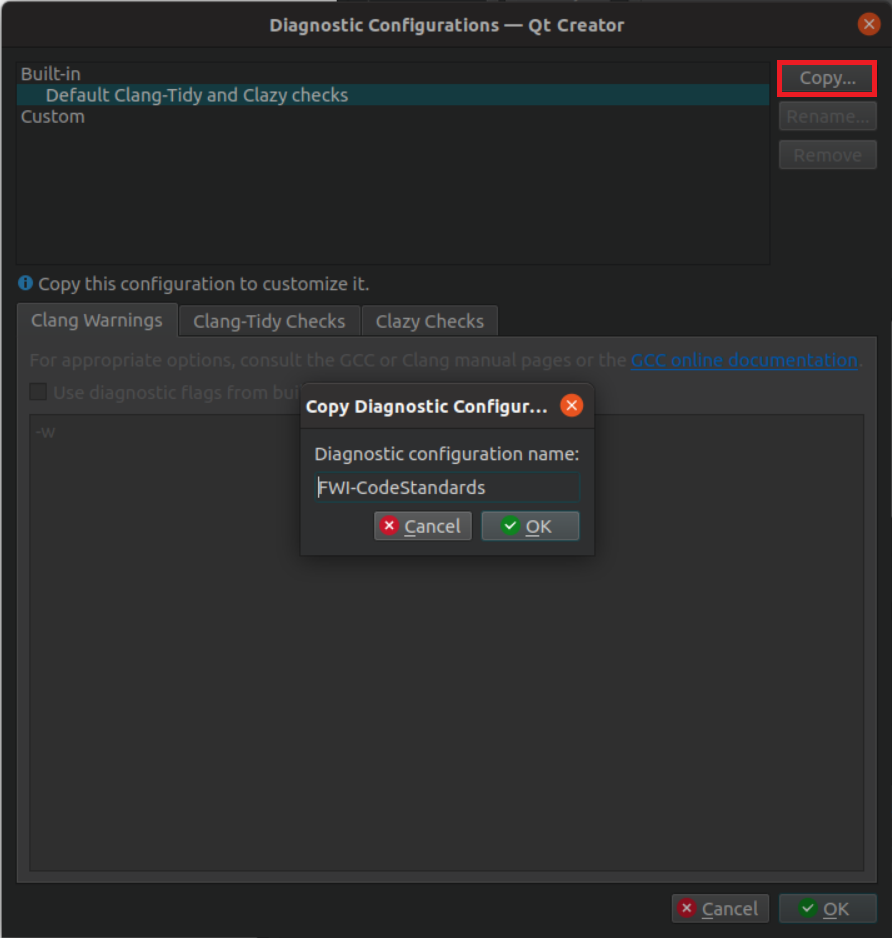
\includegraphics[width=0.6 \textwidth]{clang-tidy6.png}
\end{figure}

\item Select your own diagnostic configuration, go to the tab \textbf{Clang-Tidy Checks}, select \textbf{Use .clang-tidy config
file} in the drop-down and click \textbf{OK}.
\begin{figure}[h!]
\centering
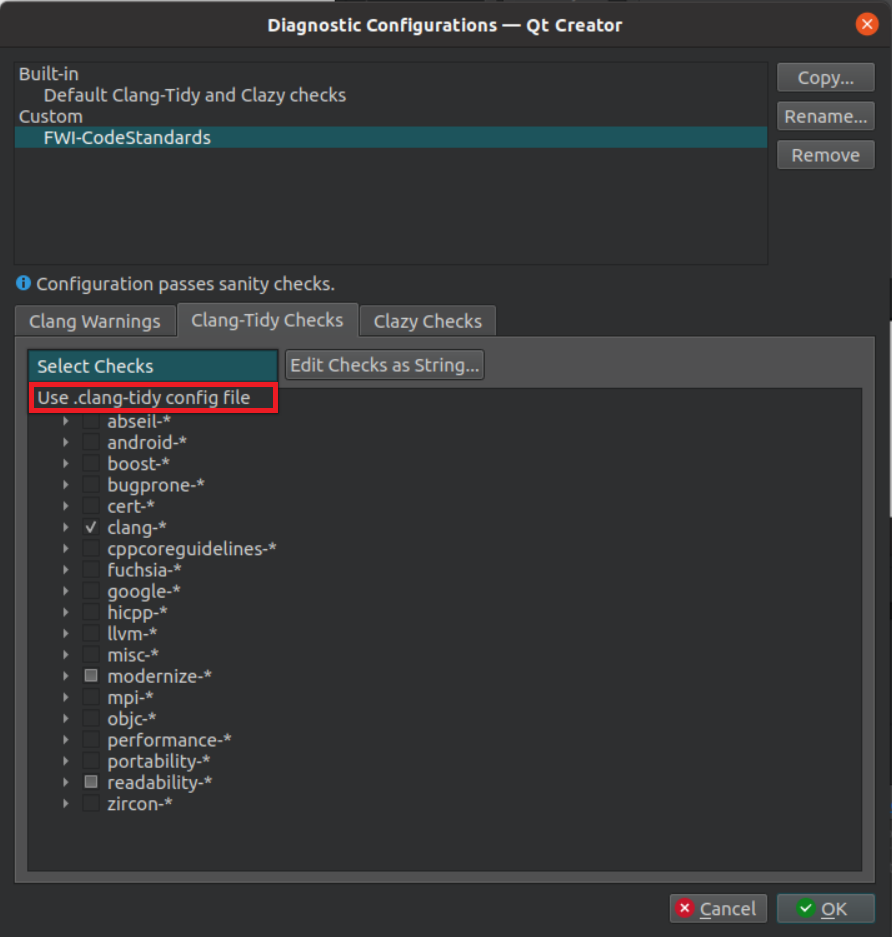
\includegraphics[width=0.6 \textwidth]{clang-tidy7.png}
\end{figure}

\newpage

\item Lastly, select the newly created diagnostic configuration in \textbf{Projects} $\rightarrow$ \textbf{Clang Tools} tab and click on \textbf{Default Clang-Tidy and Clazy checks} diagnostic configuration. Since the .clang-tidy file is already set up in the git-folder, the IDE should give warnings according to the style specified in the .clang-tidy file.
\begin{figure}[h!]
\centering
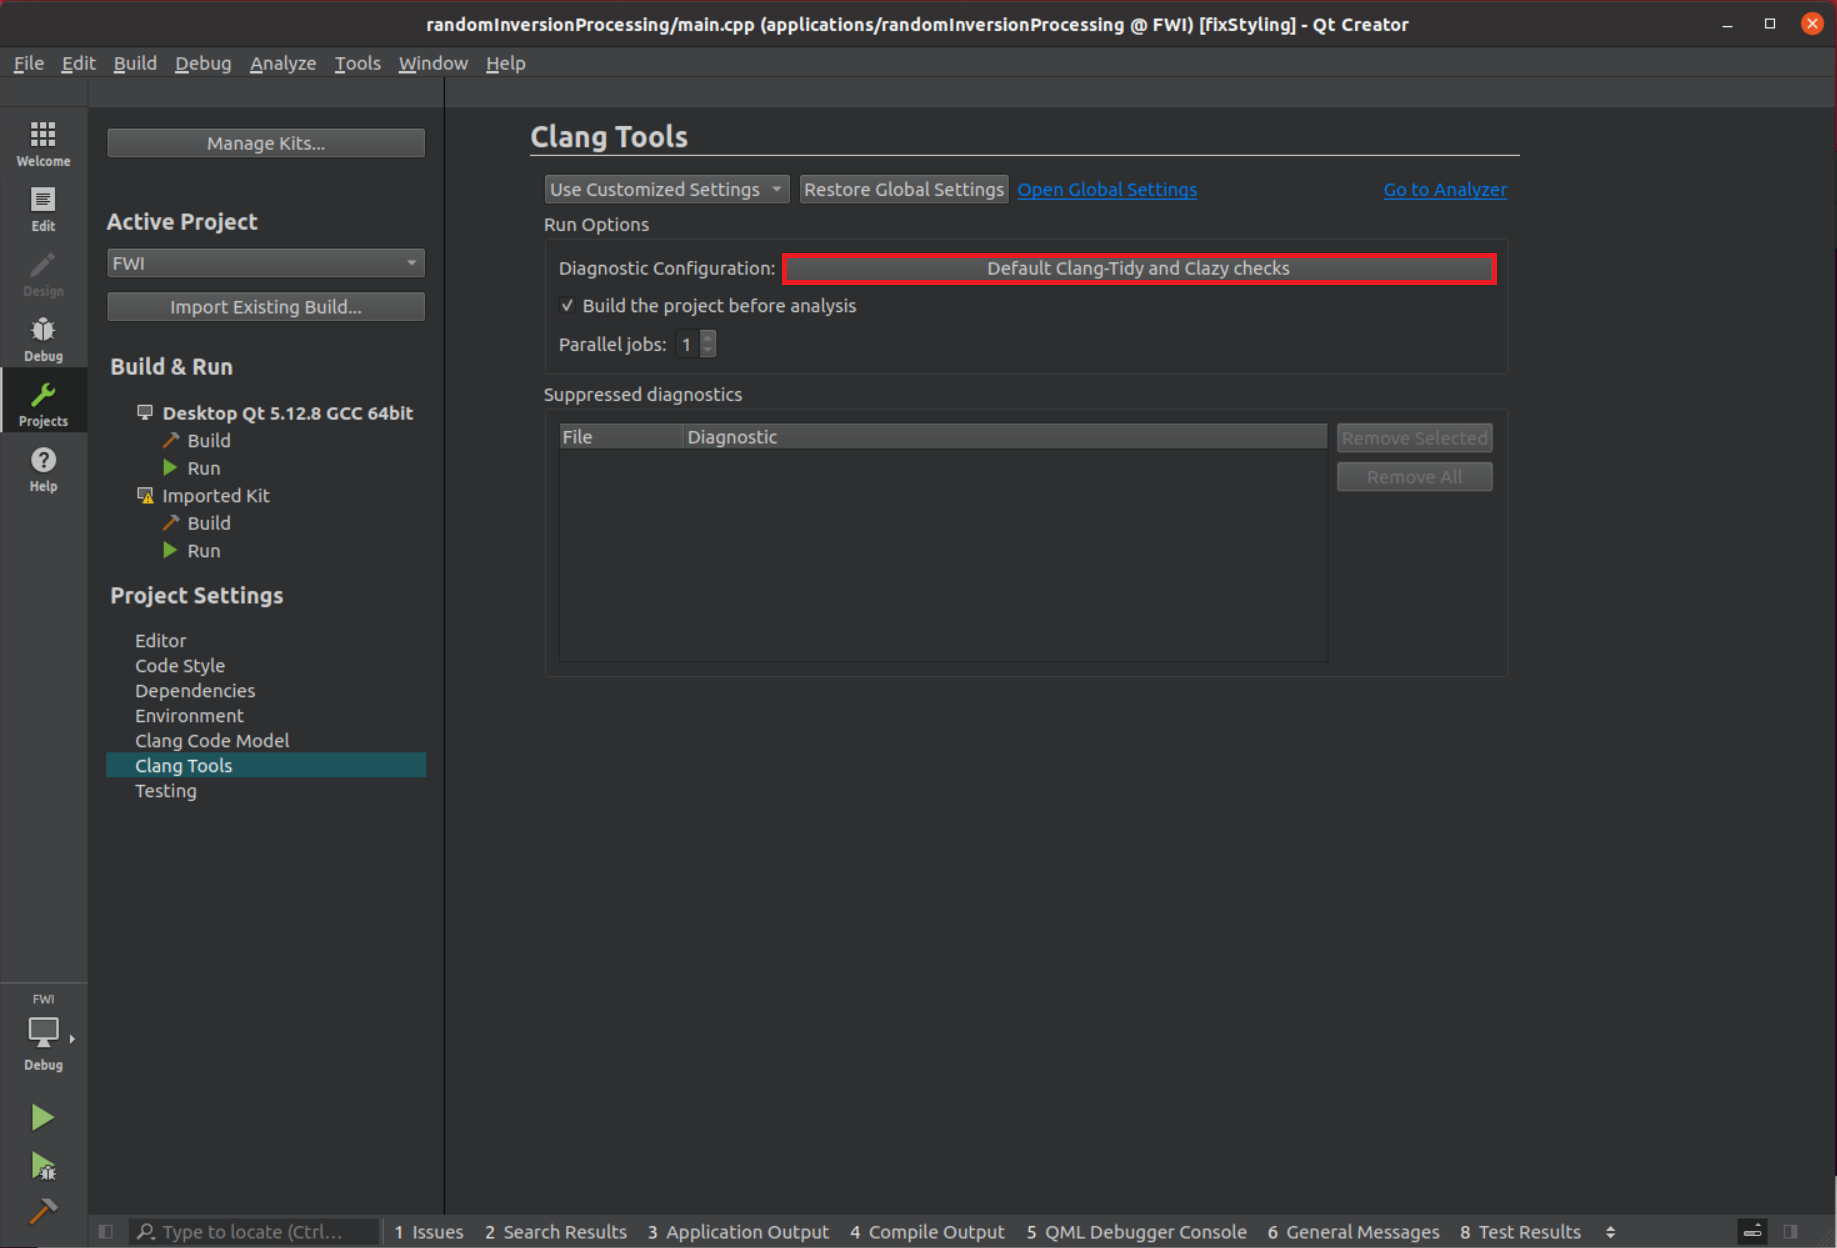
\includegraphics[width=0.65 \textwidth]{clang-tidy8.png}
\end{figure}

\item In order to run the style analysis one should select a project file and use a right mouse button click to activate the context menu. By selecting \textbf{Analyze current file} option the style checks can activated.
\begin{figure}[h!]
\centering
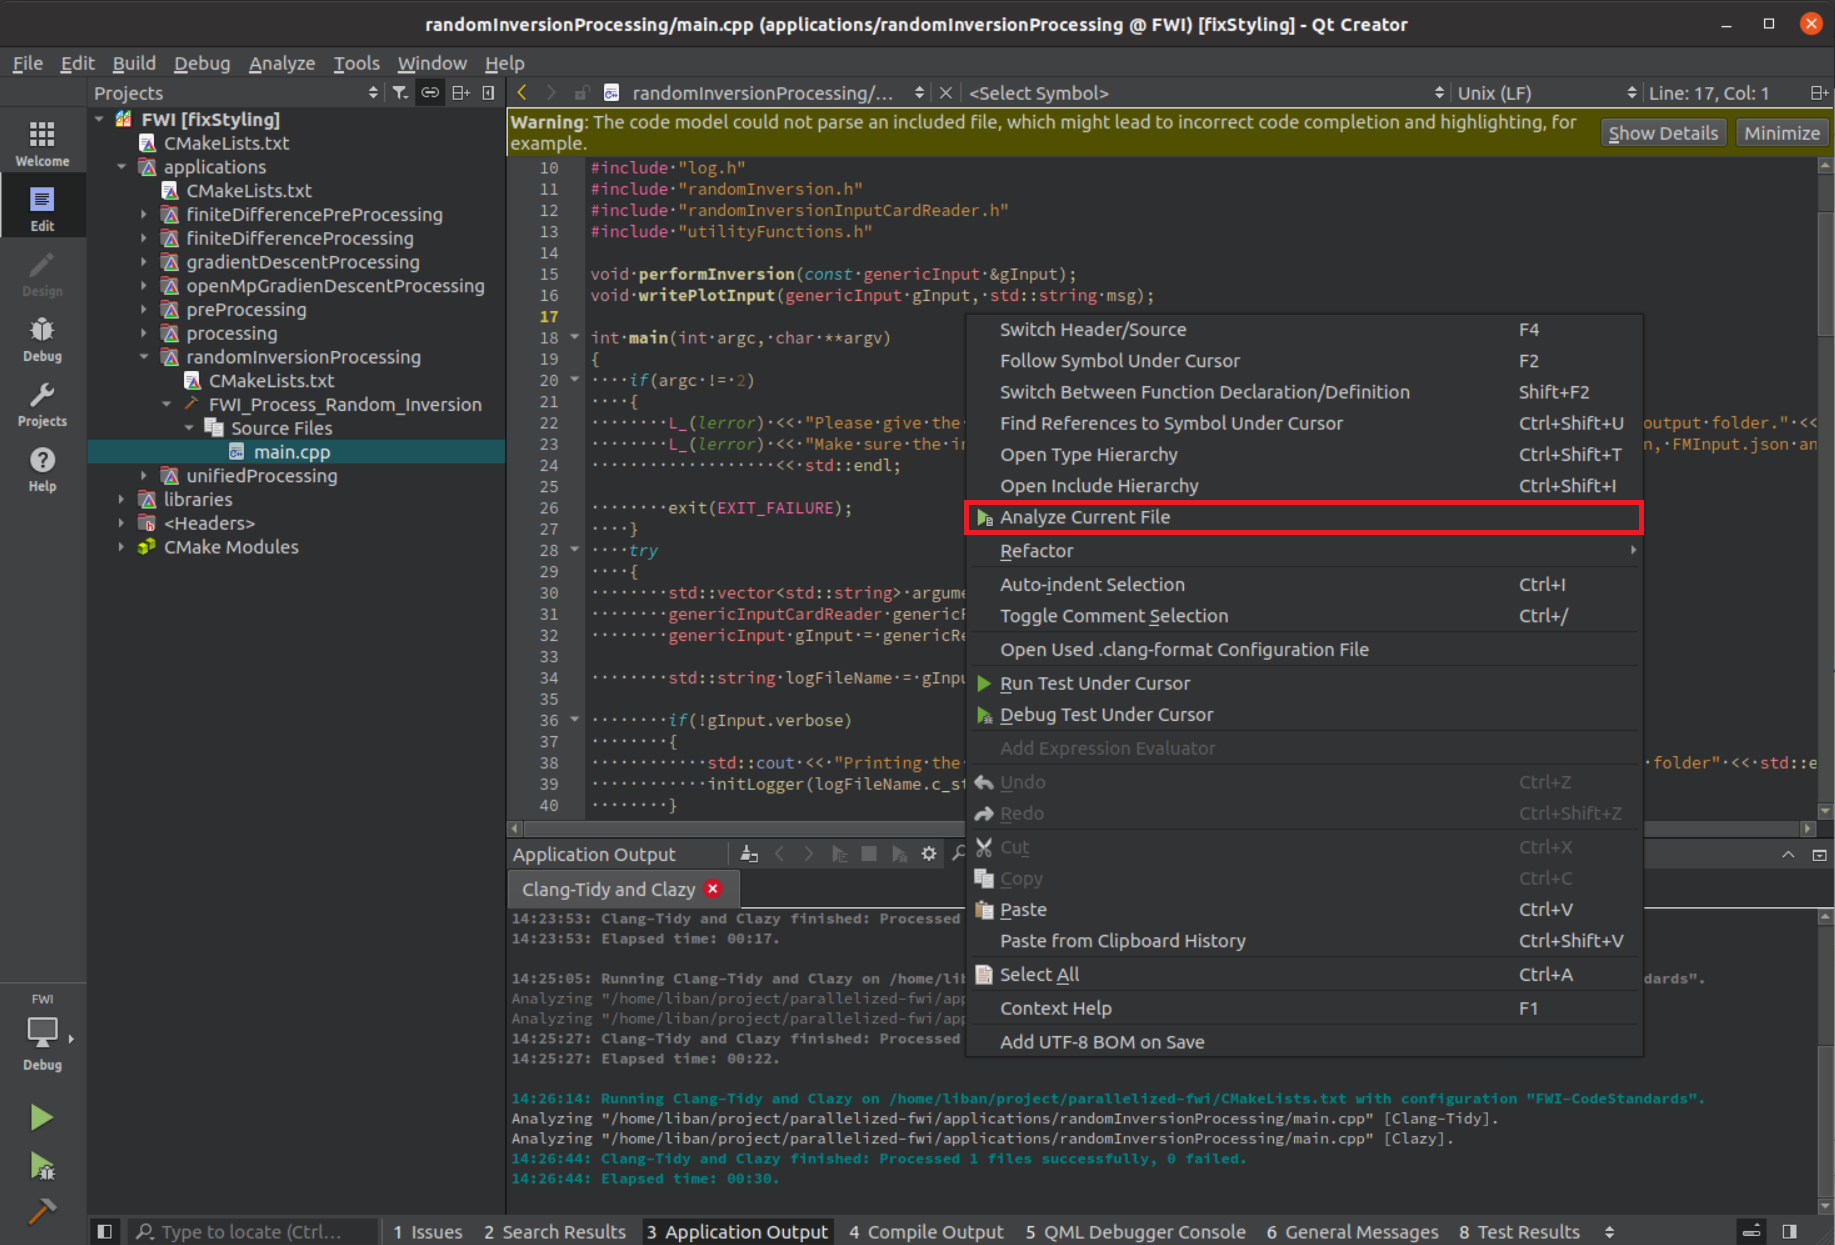
\includegraphics[width=0.65 \textwidth]{clang-tidy9.png}
\end{figure}

\newpage
\item An alternative way to run the checks on multiple files is to go to \textbf{Analyze} $\rightarrow$ \textbf{Clang-Tidy and Clazy}.
\begin{figure}[h!]
\centering
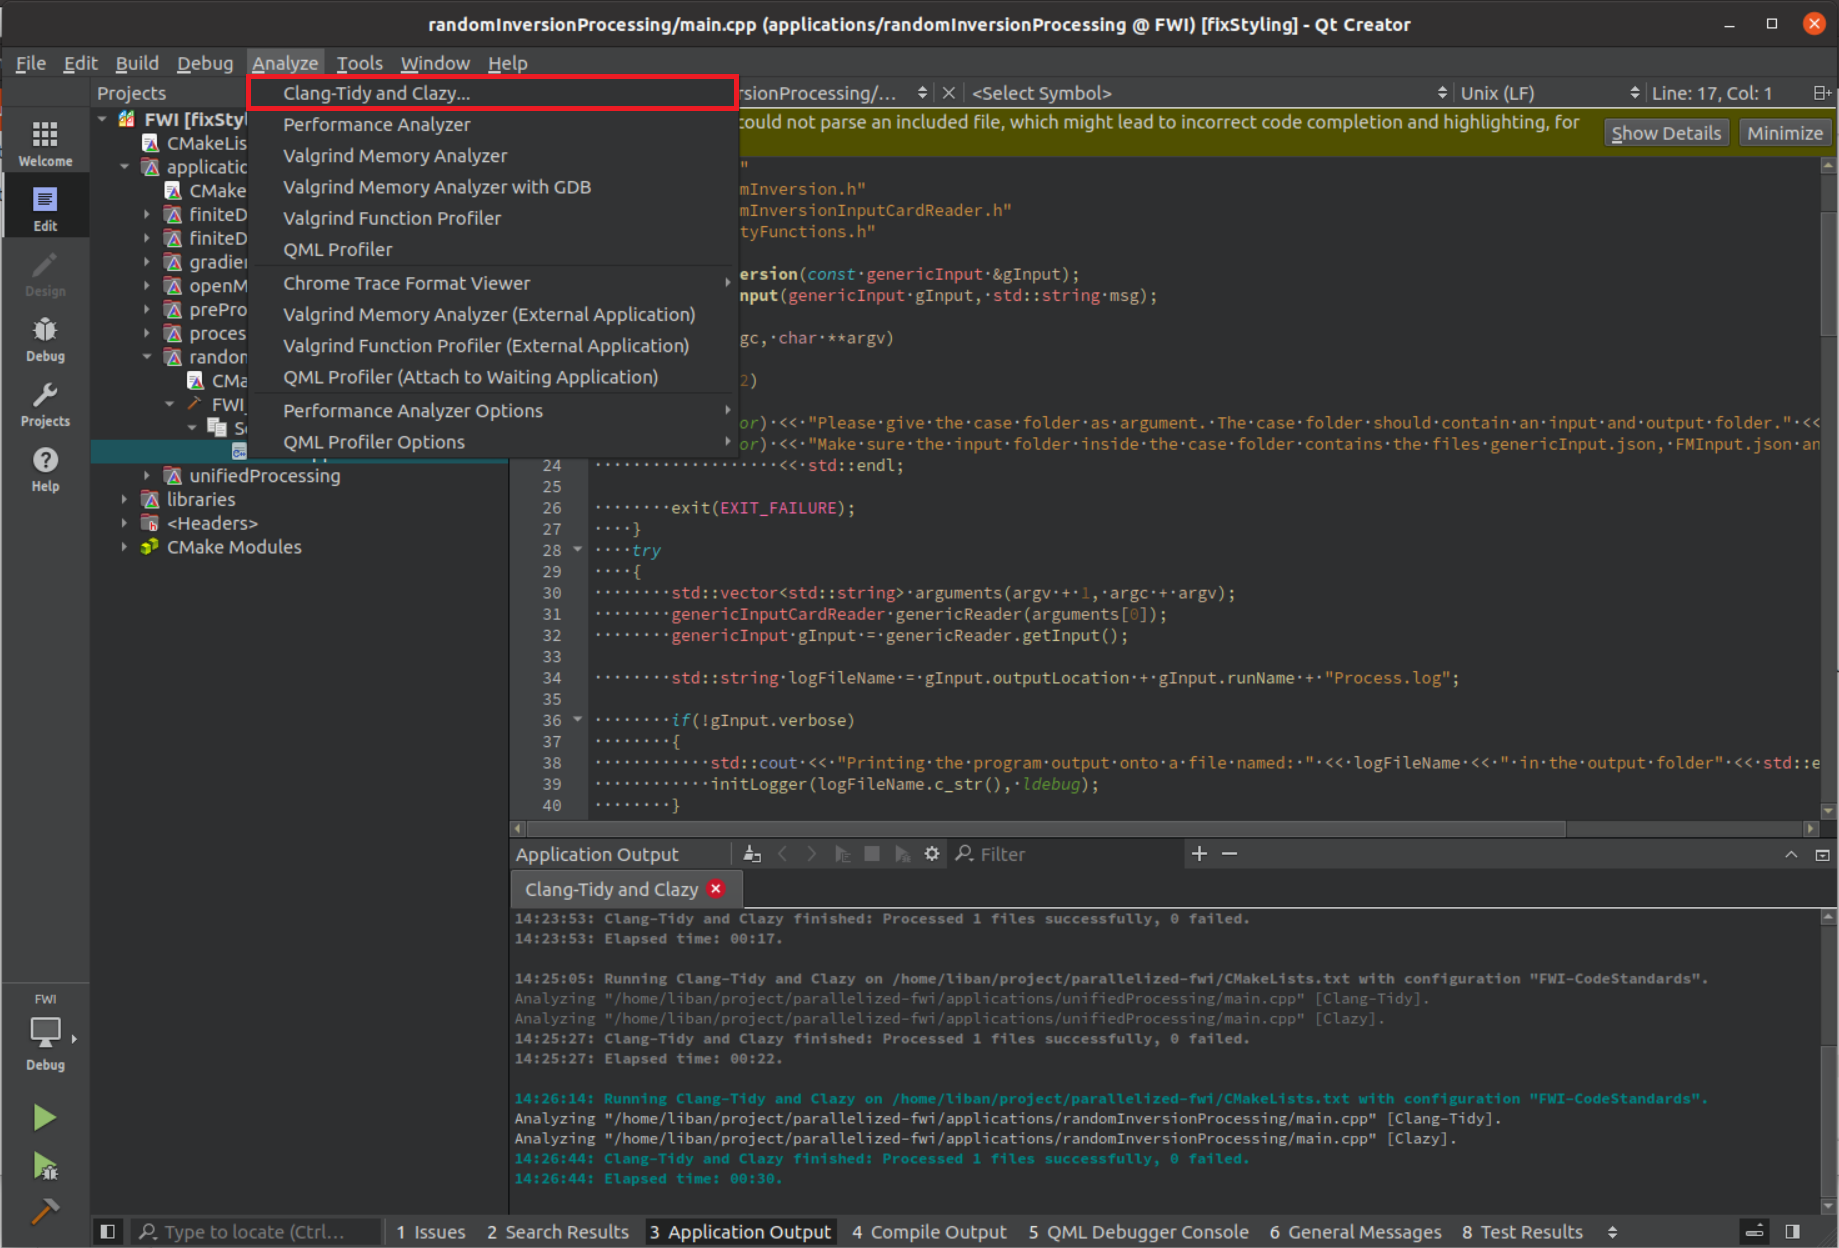
\includegraphics[width=0.6 \textwidth]{clang-tidy10.png}
\end{figure}

\item And make a final selection of the files which should be checked.
\begin{figure}[h!]
\centering
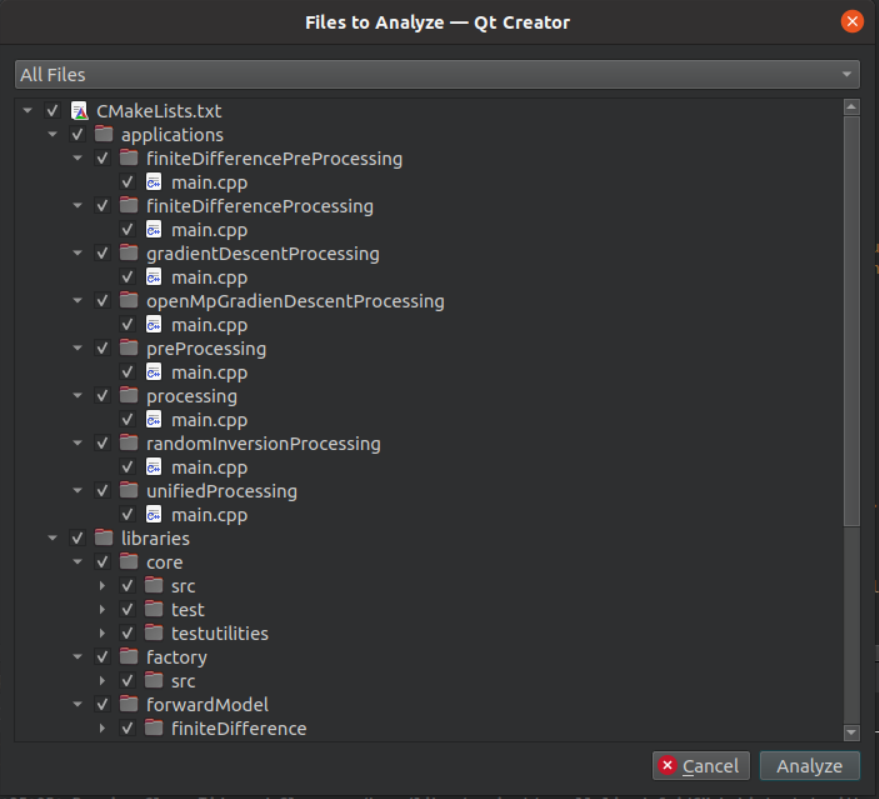
\includegraphics[width=0.6 \textwidth]{clang-tidy11.png}
\end{figure}
\end{enumerate}


\textbf{Note}: It could take a while before the clang-tidy has parsed the project and starts giving warnings.

\subsubsection*{B) Clang-tidy in other IDE's}
In other IDE’s these checks can be implemented in a similar fashion, by using the .clang-tidy configuration file.

\subsection*{Change the code-standards format}
The style used by Clang-Format is implemented in the .clang-tidy file in the parallelized-fwi folder. This file has no name, and is thus simply called .clang-tidy. In Ubuntu it is a hidden file, but it can be shown by clicking \textbf{Crtl + H}.

\end{document}

